\documentclass[11pt]{article}

% ------------------------------------------------------------
% Paquetes
% ------------------------------------------------------------
\usepackage[utf8]{inputenc}
\usepackage[T1]{fontenc}
\usepackage[spanish,es-nodecimaldot]{babel}
\usepackage{lmodern}
\usepackage{amsmath,amssymb}
\usepackage{graphicx}
\usepackage{xcolor}
\usepackage{setspace}
\usepackage{enumitem}
\usepackage{booktabs}
\usepackage{caption}
\usepackage[
    a4paper,
    margin=2.5cm
]{geometry}
\usepackage{hyperref}

% ------------------------------------------------------------
% Configuración general
% ------------------------------------------------------------
\hypersetup{
    colorlinks=true,
    linkcolor=black,
    citecolor=blue,
    urlcolor=blue,
    pdftitle={Predicción del nivel Satisfactorio en Lectura y Matemática},
    pdfauthor={Maestría en Modelización Matemática y Computacional}
}

\setstretch{1.35}
\setlist[itemize]{
    leftmargin=*,
    itemsep=2pt,
    topsep=4pt
}

\begin{document}

% ------------------------------------------------------------
% Carátula
% ------------------------------------------------------------
\begin{titlepage}
\centering

{\bfseries\large
Instituto de Matemática y Ciencias Afines -- IMCA
\par}

\vspace{0.1cm}

{\scshape\large
Maestría en Modelización Matemática y Computacional
\par}

\vspace{5.5cm}

{\bfseries\large
Trabajo de Aplicación del curso Modelamiento Estadístico Predictivo
\par}

\vspace{0.5cm}

{\Large\color{blue}
Predicción del nivel Satisfactorio en Lectura y Matemática:\\
un enfoque de clasificación aplicado a la Evaluación Muestral (EM) 2024
\par}


\vspace{1cm}


\vfill

{\large\bfseries Autores:\par}
\vspace{0.3cm}
{\large Nombre y apellidos -- Nombre y apellidos\par}

\vfill

{\large\bfseries Profesor:\par}
\vspace{0.3cm}
{\large Alex de la Cruz H.\par}

\vfill

{\large Julio de 2026\par}

\end{titlepage}

\tableofcontents

\newpage

% ------------------------------------------------------------
% Introducción
% ------------------------------------------------------------
\section{Introducción}

La Evaluación Muestral (EM) 2024, aplicada por el Ministerio de
Educación del Perú (MINEDU--UMC), mide el logro de aprendizaje de
estudiantes de sexto grado de primaria en dos competencias
fundamentales: \textbf{Lectura} y \textbf{Matemática}, clasificando a
cada estudiante en uno de cuatro niveles de desempeño (Previo al inicio,
En inicio, En proceso y Satisfactorio). Identificar qué factores
sociodemográficos, familiares y socioemocionales se asocian con alcanzar
el nivel Satisfactorio resulta clave para focalizar políticas de
refuerzo educativo de manera temprana, antes de que se apliquen
evaluaciones estandarizadas de cierre de año.

La base de datos utilizada integra tres fuentes oficiales de la EM 2024
para sexto grado de primaria, unidas mediante la llave \texttt{ID\_estudiante}
(según las llaves de cruce documentadas por MINEDU--UMC): (i) los
resultados de la evaluación (105{,}242 estudiantes a nivel nacional),
(ii) el cuestionario aplicado al propio estudiante, y (iii) el
cuestionario aplicado a la familia. De estos dos últimos se incorporan
las 40 escalas psicométricas ya construidas por MINEDU--UMC (índices
tipo Rasch/TRI) que resumen dimensiones como motivación, ansiedad
matemática, clima escolar, violencia percibida e involucramiento
parental, además de ocho variables sociodemográficas de la institución
educativa y del estudiante.

El \textbf{objetivo} de este trabajo es construir y comparar dos modelos
de clasificación binaria independientes --uno para Lectura y otro para
Matemática-- que predigan si un estudiante alcanza el nivel
Satisfactorio en cada competencia, a partir de 49 variables predictoras
sociodemográficas y socioemocionales, evaluando siete algoritmos de
clasificación bajo un mismo esquema de validación cruzada.

Contar con un modelo predictivo confiable permite a las autoridades
educativas anticipar, incluso antes de la evaluación, qué perfiles de
estudiantes tienen menor probabilidad de alcanzar el nivel esperado, y
así dirigir recursos de acompañamiento pedagógico --y no solo
económicos o de infraestructura-- de forma más eficiente.

% ------------------------------------------------------------
% Metodología
% ------------------------------------------------------------
\section{Metodología}

\subsection{Fuentes de datos y cruce}

Se integran tres bases oficiales de la EM 2024 (MINEDU--UMC): resultados
de evaluación, cuestionario al estudiante y cuestionario a la familia.
Siguiendo la nota técnica que acompaña la base de datos, la llave de
cruce entre resultados y ambos cuestionarios es \texttt{ID\_estudiante}
(las llaves para cuestionarios de docente y director, \texttt{cod\_mod7}
+ \texttt{anexo} [+ \texttt{ID\_seccion}], no se emplean por no contar
con esos archivos). El cruce alcanza una cobertura de 97.3\,\% con el
cuestionario al estudiante y 91.1\,\% con el de familia sobre el
universo de resultados; se optó por una unión (\emph{left join}) desde
la base de resultados, preservando el universo completo y añadiendo
indicadores binarios de no-respuesta a cada cuestionario como
predictores propios, en lugar de descartar a los estudiantes cuyas
familias no respondieron.

\subsection{Variables objetivo}

Se definen dos variables respuesta binarias, modeladas de forma
\textbf{independiente}:
$$Y_{lectura} = \mathbb{1}\{grupo\_L = \text{Satisfactorio}\}, \qquad
Y_{matematica} = \mathbb{1}\{grupo\_M = \text{Satisfactorio}\}$$

\subsection{Selección de variables predictoras}

Se seleccionan 49 variables: ocho sociodemográficas (área, gestión y
característica de la IE, sexo, lengua materna, índice y nivel
socioeconómico, departamento), 26 escalas compuestas del cuestionario al
estudiante y 14 del cuestionario a la familia, más dos indicadores de
no-respuesta a cada cuestionario. Se excluyen deliberadamente
\texttt{medida500\_L}/\texttt{medida500\_M} (la medida continua de la
cual se deriva determinísticamente el nivel de logro) por constituir
fuga de información. Se descartan asimismo los $\sim$170 ítems crudos de
cada cuestionario, dado que las 40 escalas compuestas ya los resumen
psicométricamente; incluir ambos simultáneamente sería redundante y
elevaría innecesariamente la dimensionalidad.

\subsection{Tratamiento de datos faltantes}

La variable \texttt{ise} presentaba 18{,}186 valores (17.3\,\%)
codificados como texto \texttt{"\#NULL!"}; se recodificaron como
faltantes reales y la variable se imputó con la mediana (\texttt{nse}
con la moda), dejando una variable indicadora de imputación. Las 40
escalas compuestas, con missing entre 2\,\% y 24\,\% según la variable
(máximo en \texttt{FAM6PGEN\_ACOSVIC}, acoso escolar), se imputaron con
su propia mediana. Se excluyen del análisis los 4{,}296 estudiantes sin
nivel de logro válido en al menos una competencia.

\subsection{Estrategia de muestreo}

Por viabilidad computacional al comparar siete algoritmos con validación
cruzada --en particular por el costo cuadrático/cúbico de SVM respecto
al número de observaciones-- se trabaja sobre una submuestra aleatoria
estratificada de 15{,}002 estudiantes, extraída del universo de 100{,}946
con nivel de logro válido. Esta decisión se documenta como limitación en
la sección correspondiente.

\subsection{División entrenamiento / prueba y modelos}

Para cada variable respuesta se realiza una partición aleatoria
estratificada 70/30. Se ajustan siete modelos por separado para Lectura
y Matemática: regresión \textbf{logística} y \textbf{probit} (enlaces
lineales de referencia); \textbf{Lasso}, \textbf{Ridge} y
\textbf{Elastic Net} (regularización L1/L2/combinada vía
\texttt{glmnet}); \textbf{SVM} con kernel radial; y \textbf{Random
Forest} (300 árboles). Todos se entrenan con validación cruzada de
$k=5$ folds maximizando el AUC-ROC promedio, vía \texttt{caret::train()}.

\subsection{Métricas de evaluación}

Sobre el conjunto de prueba se reportan exactitud, sensibilidad,
especificidad, F1-score y AUC-ROC, dado el desbalance de clases presente
en ambas variables respuesta (23.5\,\% Satisfactorio en Lectura, 14.7\,\%
en Matemática).

\subsection{Software}

R, paquetes \texttt{caret}, \texttt{glmnet}, \texttt{e1071},
\texttt{kernlab}, \texttt{randomForest}, \texttt{pROC} y \texttt{tidyverse}.

\newpage

% ------------------------------------------------------------
% Resultados
% ------------------------------------------------------------
\section{Resultados}

\subsection{Descripción general de la base de datos}

La base de resultados contiene 105{,}242 estudiantes a nivel nacional.
Tras excluir registros sin nivel de logro válido en alguna competencia
quedan 100{,}946 estudiantes, de los cuales se extrae la submuestra de
trabajo de 15{,}002 casos. En esta submuestra, el 23.45\,\% de los
estudiantes alcanza el nivel Satisfactorio en Lectura y el 14.72\,\% en
Matemática --un desbalance de clases relevante que se retoma en la
interpretación de resultados.

\subsection{Análisis exploratorio}

Se observa un gradiente socioeconómico claro: la proporción de
estudiantes que alcanza el nivel Satisfactorio crece de forma sostenida
del nivel socioeconómico bajo al alto, tanto en Lectura como en
Matemática. A nivel de las escalas socioemocionales, variables como la
ansiedad ante la matemática y la motivación hacia la matemática muestran
diferencias visibles en su distribución entre quienes alcanzan el nivel
Satisfactorio y quienes no, particularmente para la competencia de
Matemática.

\subsection{Preprocesamiento}

Las variables categóricas se codifican como variables \emph{dummy}
dentro de \texttt{caret::train()} para los modelos que lo requieren
(\texttt{glmnet}, \texttt{svmRadial}); las variables numéricas se
centran y escalan únicamente para SVM. Los modelos basados en árboles y
los GLM no requieren estandarización.

\subsection{Entrenamiento y validación: hiperparámetros seleccionados}

La Tabla~\ref{tab:hiperparam} resume los hiperparámetros óptimos
seleccionados por validación cruzada para cada modelo y competencia.

\begin{table}[h]
\centering
\small
\begin{tabular}{lcccc}
\toprule
\textbf{Modelo} & \textbf{Hiperparámetro} & \textbf{Lectura} & \textbf{Matemática} \\
\midrule
Lasso        & $\lambda$        & 0.0004 & 0.0007 \\
Ridge        & $\lambda$        & 0.0078 & 0.0078 \\
Elastic Net  & $\alpha$ / $\lambda$ & 0.5 / 0.0008 & 0.9 / 0.0008 \\
SVM radial   & $\sigma$ / $C$   & 0.0074 / 0.50 & 0.0074 / 0.25 \\
Random Forest & mtry            & 27     & 2      \\
\bottomrule
\end{tabular}
\caption{Hiperparámetros óptimos seleccionados por validación cruzada ($k=5$)}
\label{tab:hiperparam}
\end{table}

\subsection{Tabla comparativa de desempeño}

Las Tablas~\ref{tab:lectura} y~\ref{tab:matematica} presentan las
métricas de desempeño de los siete modelos sobre el conjunto de prueba,
para Lectura y Matemática respectivamente.

\begin{table}[h]
\centering
\small
\begin{tabular}{lccccc}
\toprule
\textbf{Modelo} & \textbf{Accuracy} & \textbf{Sensibilidad} & \textbf{Especificidad} & \textbf{F1} & \textbf{AUC} \\
\midrule
Probit       & 0.806 & 0.396 & 0.931 & 0.489 & \textbf{0.826} \\
Logit        & 0.806 & 0.405 & 0.929 & 0.494 & \textbf{0.826} \\
Lasso        & 0.806 & 0.397 & 0.931 & 0.490 & \textbf{0.826} \\
Elastic Net  & 0.806 & 0.397 & 0.932 & 0.490 & \textbf{0.826} \\
Ridge        & 0.805 & 0.369 & 0.938 & 0.470 & 0.823 \\
Random Forest & 0.797 & 0.275 & 0.957 & 0.388 & 0.804 \\
SVM          & --    & --    & --    & --    & sin convergencia$^{*}$ \\
\bottomrule
\end{tabular}
\caption{Comparación de modelos --- Lectura (conjunto de prueba, n$\approx$4{,}500)}
\label{tab:lectura}
\end{table}

\begin{table}[h]
\centering
\small
\begin{tabular}{lccccc}
\toprule
\textbf{Modelo} & \textbf{Accuracy} & \textbf{Sensibilidad} & \textbf{Especificidad} & \textbf{F1} & \textbf{AUC} \\
\midrule
Probit       & 0.863 & 0.218 & 0.974 & 0.319 & \textbf{0.833} \\
Logit        & 0.863 & 0.237 & 0.971 & 0.338 & 0.832 \\
Lasso        & 0.863 & 0.221 & 0.973 & 0.321 & 0.832 \\
Elastic Net  & 0.862 & 0.218 & 0.974 & 0.318 & 0.832 \\
Ridge        & 0.862 & 0.201 & 0.977 & 0.301 & 0.829 \\
Random Forest & 0.853 & 0.003 & 1.000 & 0.006 & 0.799 \\
SVM          & 0.863 & 0.208 & 0.976 & 0.309 & 0.798 \\
\bottomrule
\end{tabular}
\caption{Comparación de modelos --- Matemática (conjunto de prueba, n$\approx$4{,}500)}
\label{tab:matematica}
\end{table}

\footnotesize{$^{*}$Para Lectura, el modelo SVM no produjo predicciones
de clase estables sobre el conjunto de prueba con los hiperparámetros
seleccionados por validación cruzada, por lo que sus métricas no son
reportables; se documenta como limitación.}
\normalsize

\begin{figure}[h]
\centering
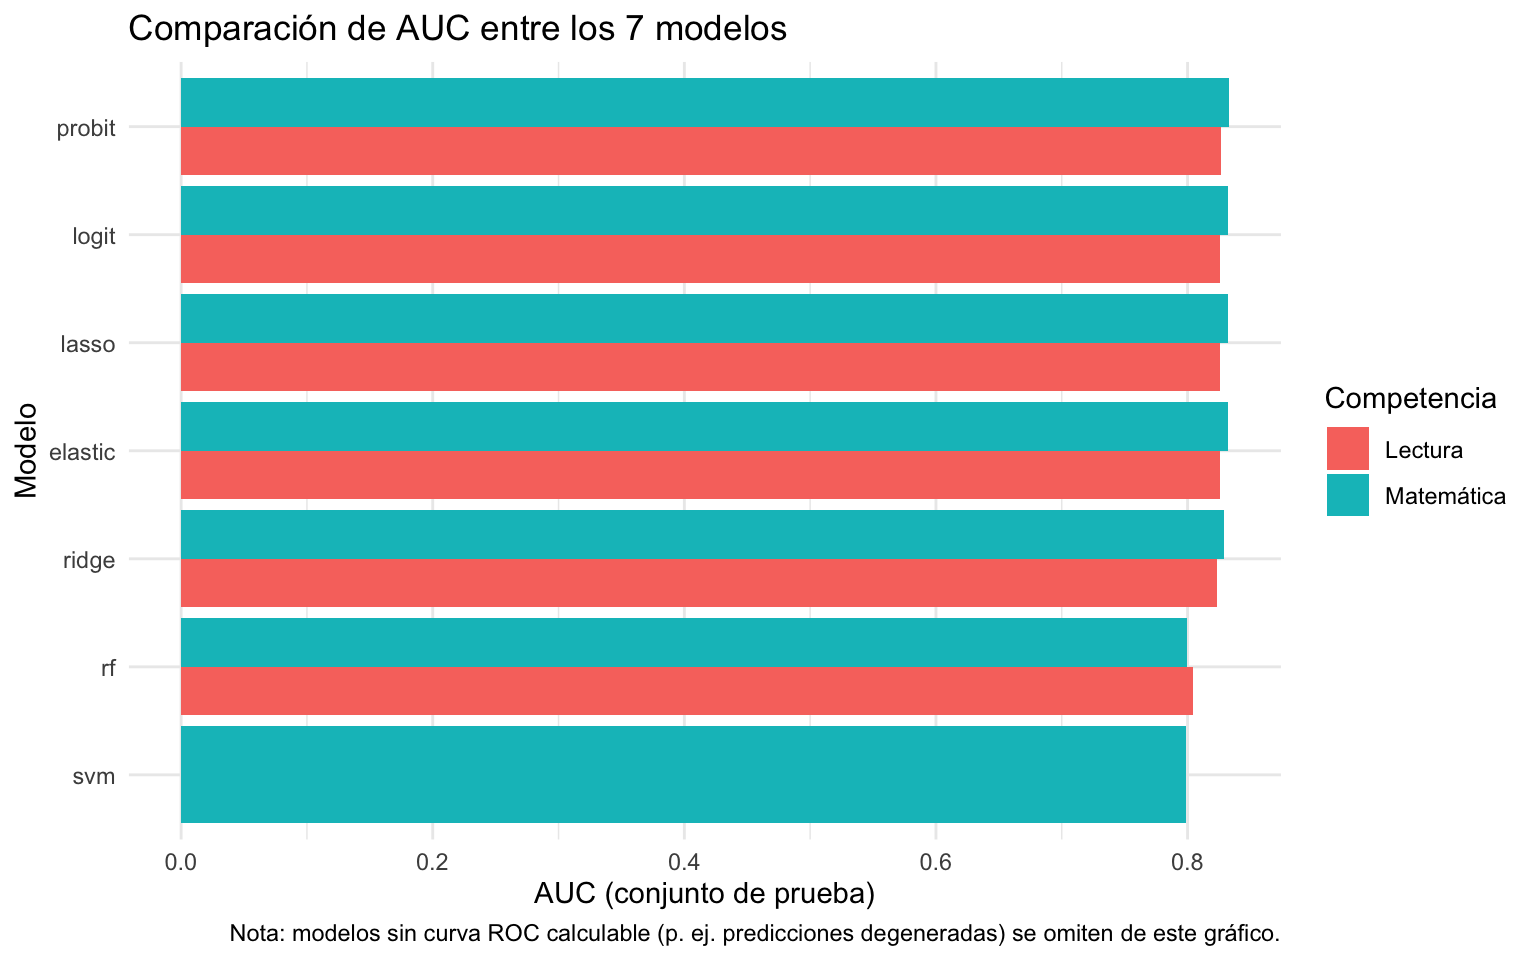
\includegraphics[width=0.85\textwidth]{figuras/fig_auc_comparativo.png}
\caption{Comparación de AUC entre los modelos evaluables, Lectura vs. Matemática}
\label{fig:auc}
\end{figure}

\newpage

\begin{figure}[h]
\centering
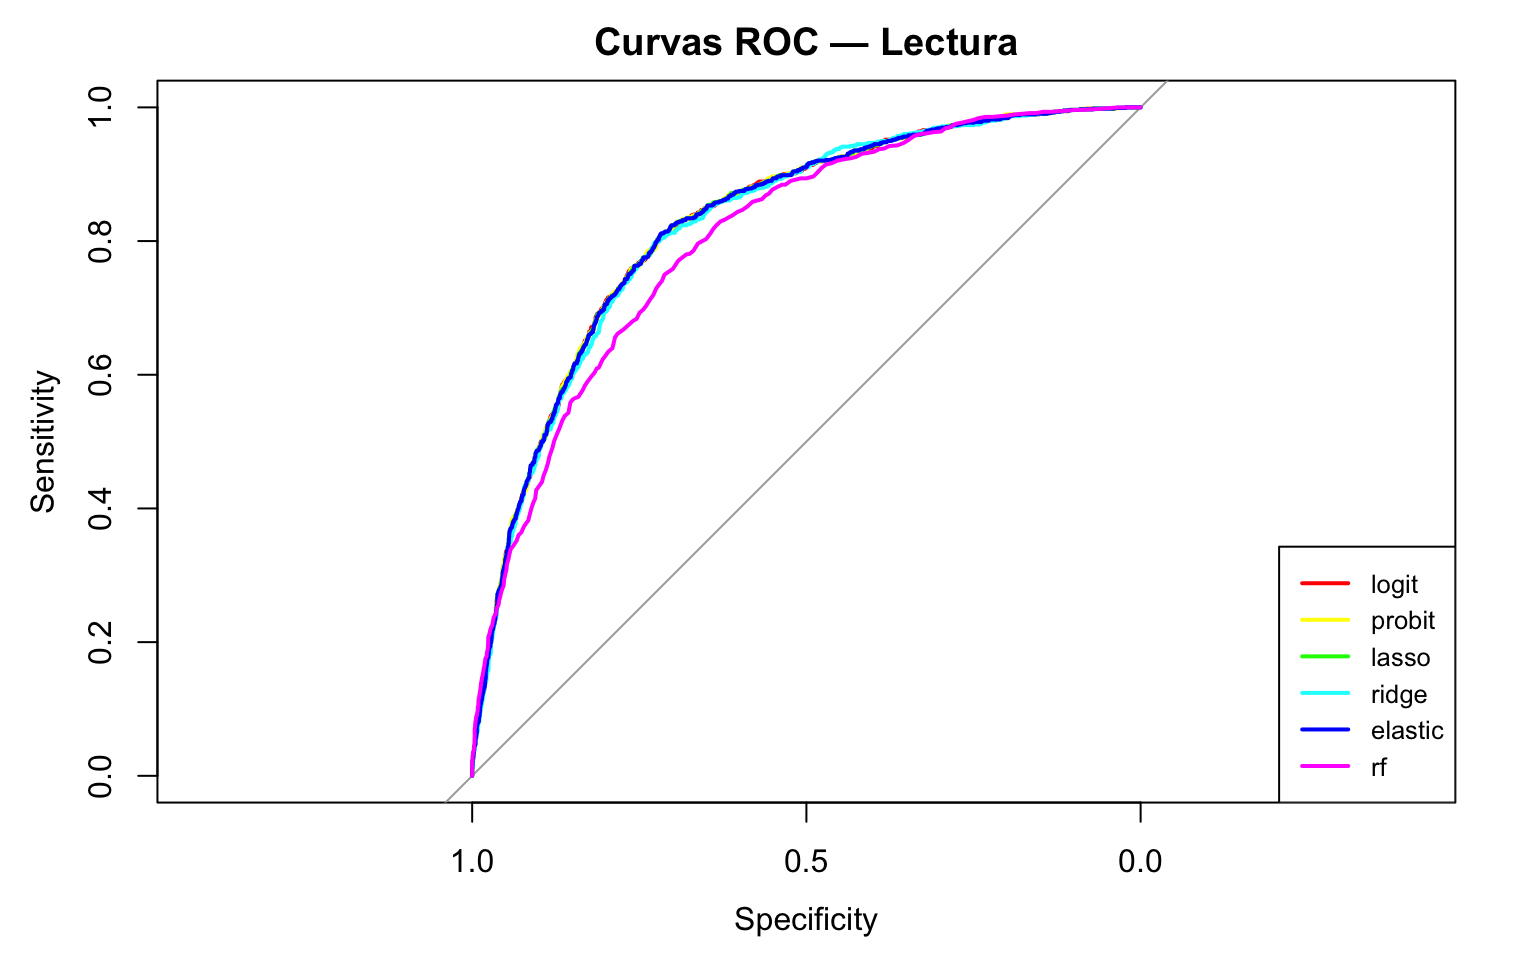
\includegraphics[width=0.8\textwidth]{figuras/fig_roc_lectura.png}
\caption{Curvas ROC de los modelos con predicción estable --- Lectura}
\label{fig:roc_lectura}
\end{figure}

\begin{figure}[h]
\centering
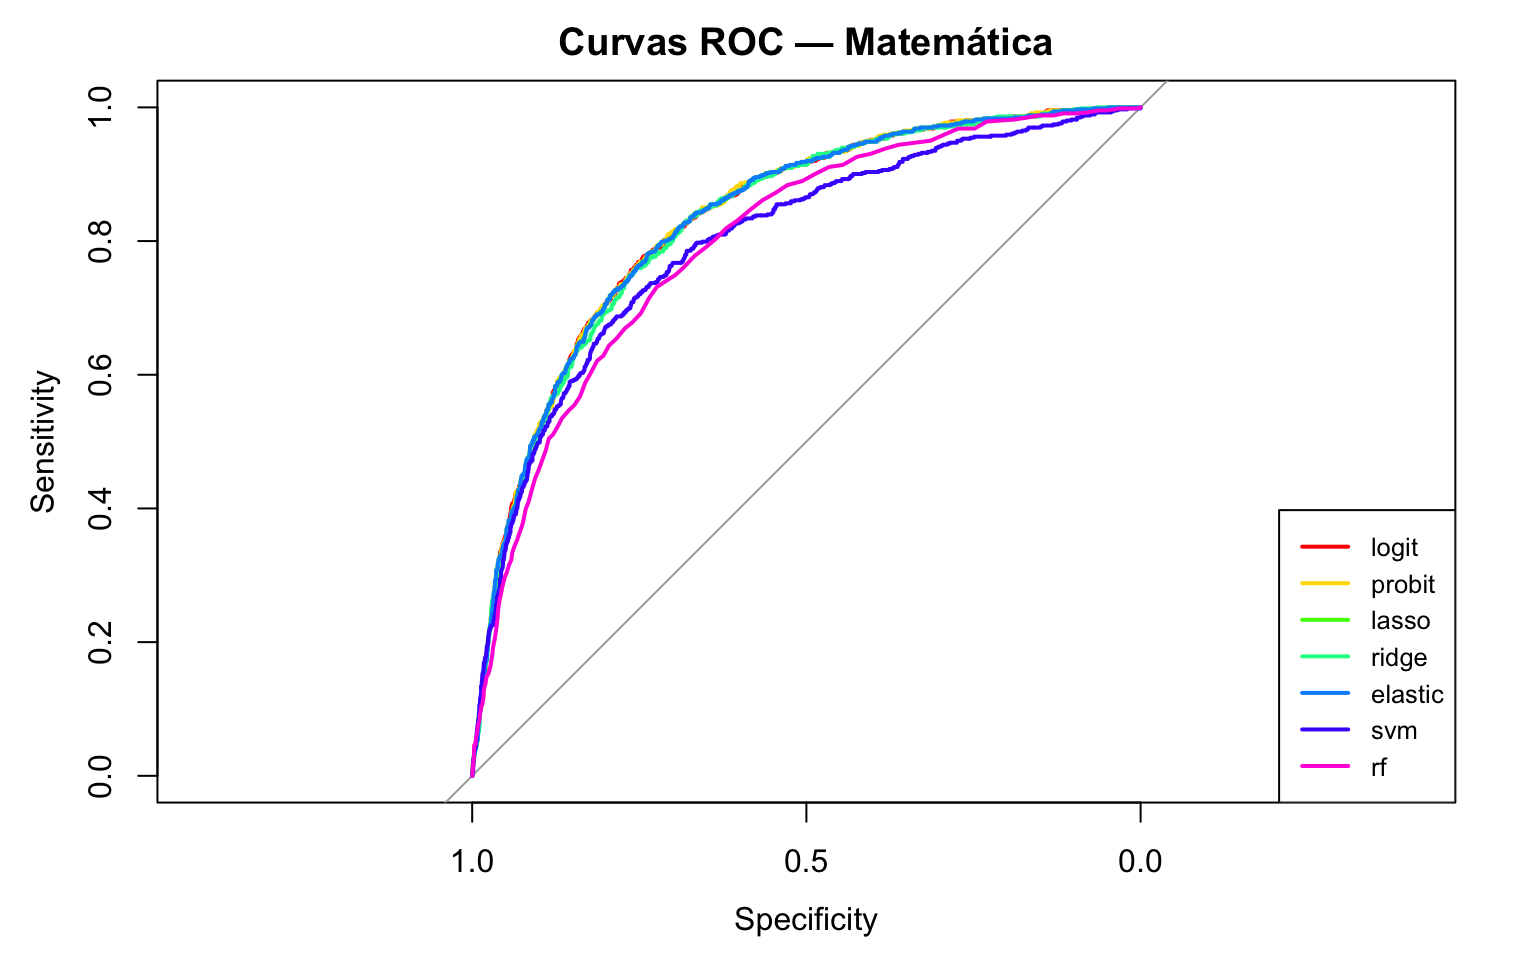
\includegraphics[width=0.8\textwidth]{figuras/fig_roc_matematica.png}
\caption{Curvas ROC de los siete modelos --- Matemática}
\label{fig:roc_matematica}
\end{figure}

\subsection{Identificación y justificación del modelo seleccionado}

Considerando el AUC como criterio principal --por ser robusto al
desbalance de clases-- y el balance entre sensibilidad y especificidad,
se selecciona la \textbf{regresión logística} como modelo final para
ambas competencias: obtiene un desempeño estadísticamente equivalente al
de los modelos regularizados (que no aportan mejora relevante,
sugiriendo baja multicolinealidad efectiva tras la selección de
variables), la mejor sensibilidad entre los modelos con AUC máximo, y
coeficientes directamente interpretables para el análisis de política
educativa. Random Forest y SVM, pese a su mayor flexibilidad, no
superan a los modelos lineales en este problema --y muestran
sensibilidad muy baja o nula, afectados por el desbalance de clases.

\subsection{Importancia de variables}

\begin{figure}[h]
\centering
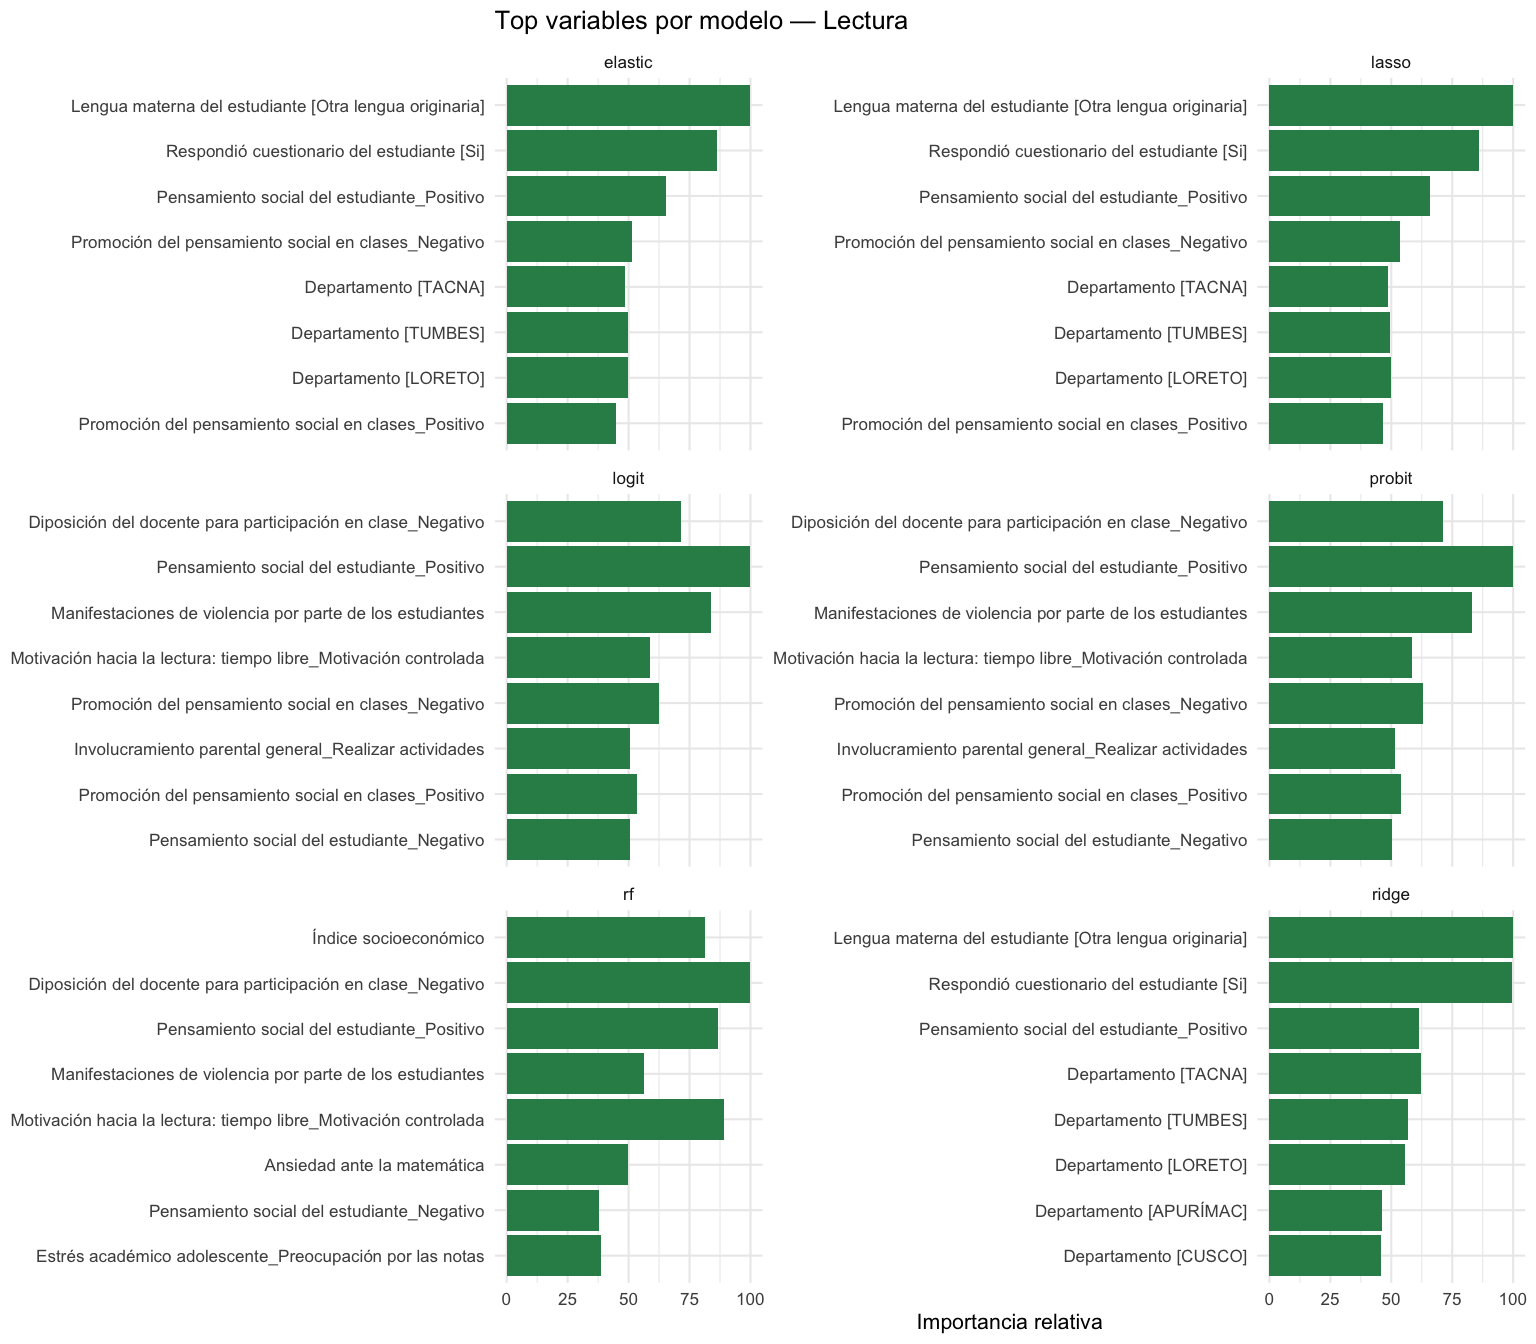
\includegraphics[width=0.95\textwidth]{figuras/fig_importancia_lectura.png}
\caption{Importancia de variables por modelo --- Lectura}
\label{fig:imp_lectura}
\end{figure}

\begin{figure}[h]
\centering
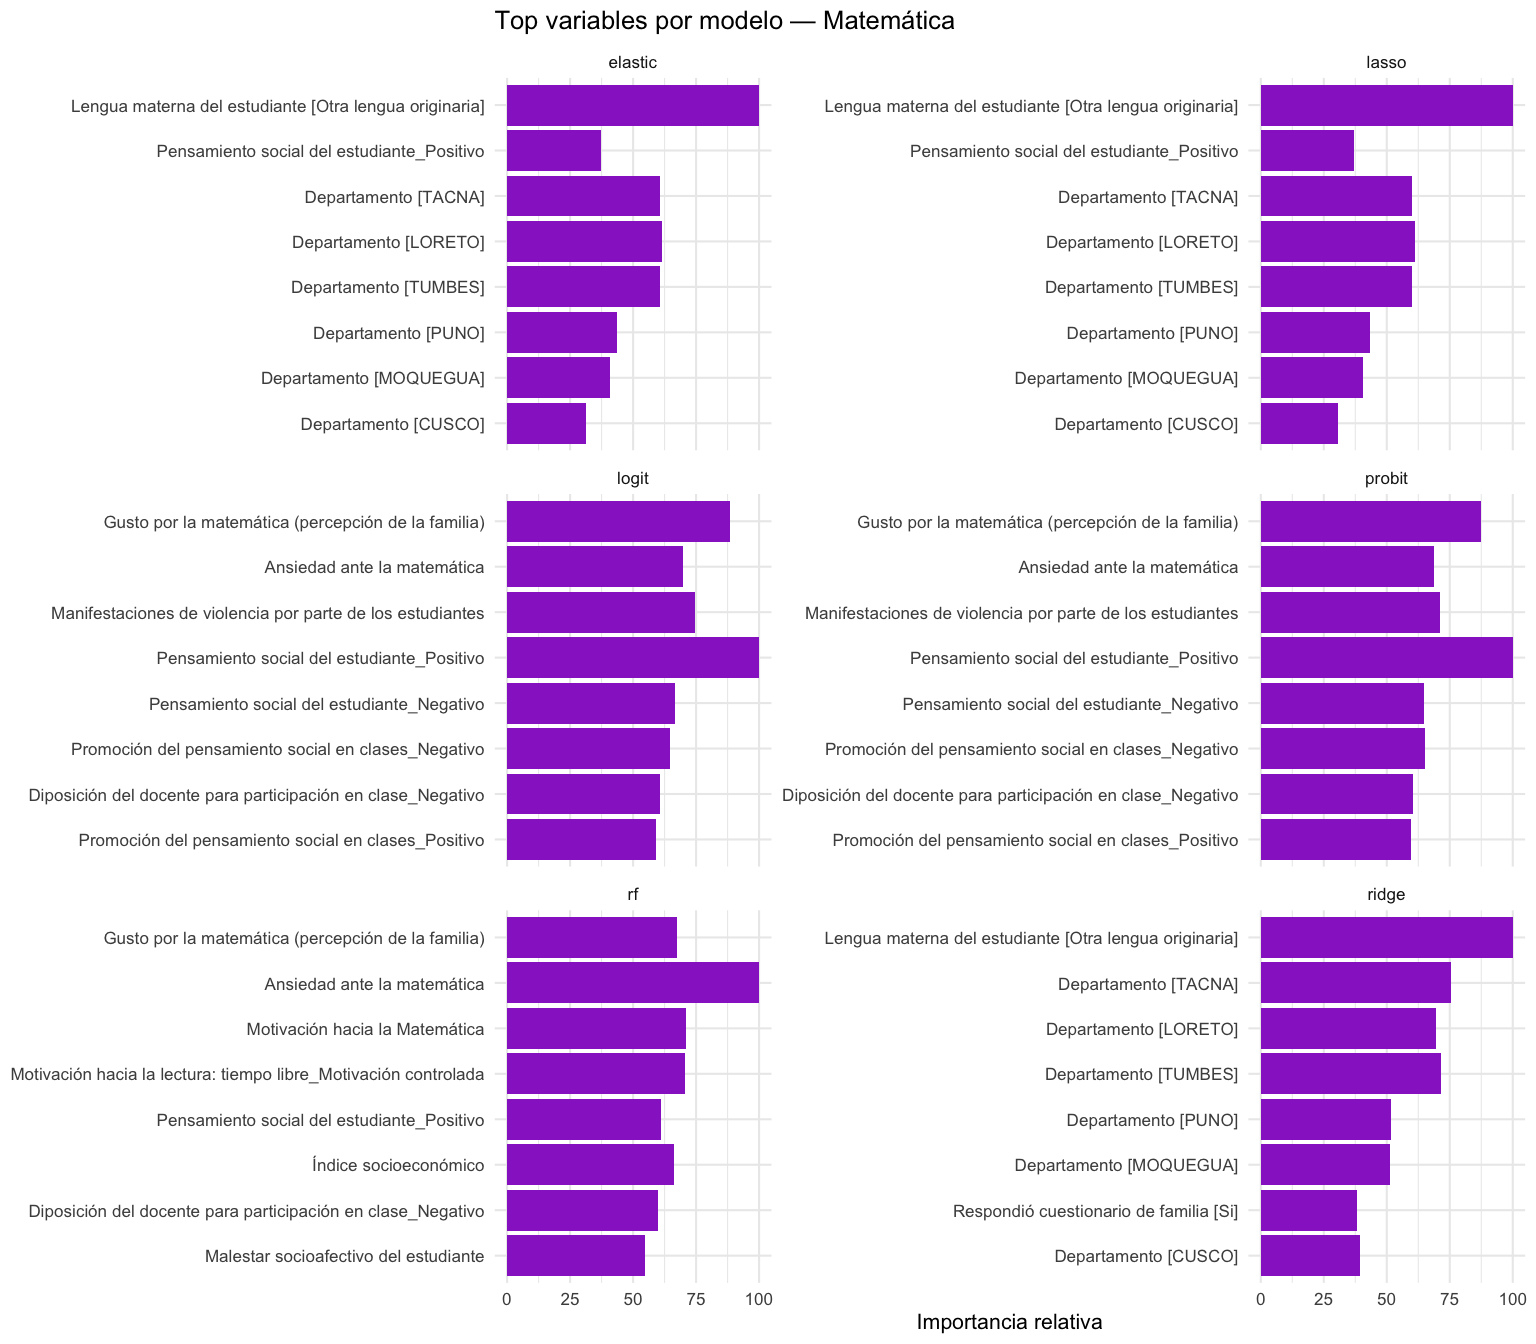
\includegraphics[width=0.95\textwidth]{figuras/fig_importancia_matematica.png}
\caption{Importancia de variables por modelo --- Matemática}
\label{fig:imp_matematica}
\end{figure}

Para \textbf{Lectura}, las variables con mayor peso en el modelo
logístico son: pensamiento social positivo del estudiante,
manifestaciones de violencia por parte de los estudiantes, disposición
negativa del docente para la participación en clase, promoción del
pensamiento social en el aula, y motivación controlada hacia la lectura
en el tiempo libre. En el modelo de Random Forest destaca además el
índice socioeconómico como cuarto predictor más relevante. En los
modelos regularizados (Lasso), la lengua materna (categoría "otra
lengua originaria") y el hecho de no haber respondido el cuestionario
del estudiante emergen como los predictores de mayor magnitud, junto con
variación relevante por departamento (Loreto, Tumbes, Tacna).

Para \textbf{Matemática}, el patrón es más específico al dominio: la
\textbf{ansiedad ante la matemática} y la \textbf{motivación hacia la
matemática} son, de forma consistente entre el modelo logístico y
Random Forest, los predictores más importantes, seguidos por el gusto
por la matemática percibido por la familia y el pensamiento social
positivo del estudiante. Este resultado es coherente con la literatura
de psicología educativa sobre ansiedad matemática como barrera
específica de aprendizaje, distinta de los determinantes más generales
de Lectura.

\subsection{Limitaciones observadas}

\begin{itemize}
    \item El \textbf{desbalance de clases} (23.5\,\% / 14.7\,\% Satisfactorio)
    limita la sensibilidad de Random Forest y, en Lectura, impidió que
    SVM produjera predicciones estables; técnicas de balanceo o ajuste
    del umbral de decisión podrían mejorar estos modelos.
    \item El uso de una \textbf{submuestra de 15{,}002} estudiantes (de
    100{,}946 disponibles) por viabilidad computacional limita la
    potencia estadística respecto de usar el universo completo.
    \item El AUC máximo alcanzado ($\approx$0.83) indica que, incluso
    con 49 predictores incluyendo escalas socioemocionales validadas,
    persiste una proporción relevante de variabilidad no explicada por
    estas variables --consistente con la naturaleza multicausal del
    aprendizaje.
    \item Los resultados corresponden a una evaluación de un año (2024)
    y son asociativos, no permiten inferir causalidad.
\end{itemize}

\newpage

% ------------------------------------------------------------
% Comentarios finales
% ------------------------------------------------------------
\section{Comentarios finales}

El objetivo planteado --predecir si un estudiante alcanza el nivel
Satisfactorio en Lectura y en Matemática mediante dos modelos binarios
independientes-- se cumple: la regresión logística ofrece el mejor
balance entre desempeño e interpretabilidad para ambas competencias, con
un AUC de prueba de 0.826 en Lectura y 0.832 en Matemática, superando de
forma consistente a Random Forest y SVM bajo el desbalance de clases
observado.

Un hallazgo sustantivo de este trabajo es que las \textbf{escalas
socioemocionales y de clima escolar} --construidas a partir de los
cuestionarios al estudiante y a la familia-- añaden una capacidad
predictiva considerable respecto de usar únicamente variables
sociodemográficas: la ansiedad y motivación hacia la matemática, el
clima de violencia percibida en el aula y el involucramiento parental
resultan tan o más relevantes que el índice socioeconómico, que
dominaba como predictor principal en una primera versión del análisis
restringida a variables sociodemográficas. Esto sugiere que las
intervenciones de refuerzo educativo no deberían limitarse a criterios
puramente económicos, sino considerar también el bienestar
socioemocional del estudiante y su relación con el aula.

El modelo seleccionado tiene utilidad práctica principalmente como
herramienta de \textbf{priorización}, no de decisión individual: permite
ordenar a los estudiantes según su probabilidad estimada de no alcanzar
el nivel Satisfactorio, apoyando la focalización de recursos --tanto
académicos como socioemocionales-- hacia los perfiles de mayor riesgo.

Como principales limitaciones se señalan el desbalance de clases no
corregido, el uso de una submuestra por razones computacionales, y la
falta de las variables de los cuestionarios a docentes y directores (no
disponibles para este trabajo), que podrían capturar el efecto del aula
y la institución educativa. Como líneas futuras se propone: (i) aplicar
técnicas de balanceo de clases (SMOTE, ponderación por costos) y
optimización del umbral de decisión, especialmente para resolver la
inestabilidad de SVM en Lectura; (ii) incorporar los cuestionarios de
docente y director mediante sus llaves oficiales de cruce; y (iii)
explorar modelos multinivel que consideren el efecto de la institución
educativa sobre el desempeño de sus estudiantes.

% ------------------------------------------------------------
% Referencias
% ------------------------------------------------------------
\section*{Referencias}
\addcontentsline{toc}{section}{Referencias}

\begin{itemize}
    \item Ministerio de Educación del Perú -- UMC. (2024). \textit{Evaluación
    Muestral (EM) 2024, Sexto Grado de Primaria}. Bases de datos
    innominadas: resultados, cuestionario al estudiante y cuestionario a
    la familia.
    \item Kuhn, M. (2008). Building predictive models in R using the
    caret package. \textit{Journal of Statistical Software}, 28(5), 1--26.
    \item Friedman, J., Hastie, T., \& Tibshirani, R. (2010).
    Regularization paths for generalized linear models via coordinate
    descent. \textit{Journal of Statistical Software}, 33(1), 1--22.
    \item Breiman, L. (2001). Random forests. \textit{Machine Learning},
    45(1), 5--32.
    \item Cortes, C., \& Vapnik, V. (1995). Support-vector networks.
    \textit{Machine Learning}, 20(3), 273--297.
\end{itemize}

% ------------------------------------------------------------
% Anexos
% ------------------------------------------------------------
\appendix
\section{Anexos}

\subsection{Diccionario de escalas compuestas más relevantes}

\begin{table}[h]
\centering
\footnotesize
\begin{tabular}{ll}
\toprule
\textbf{Código} & \textbf{Descripción} \\
\midrule
EST6PCCSS\_PENSOCPO & Pensamiento social del estudiante -- Positivo \\
EST6PGEN\_VIOLEST   & Manifestaciones de violencia por parte de los estudiantes \\
EST6PGEN\_OPARDOCN  & Disposición negativa del docente para participación en clase \\
EST6PMAT\_ANSIE     & Ansiedad ante la matemática \\
EST6PMAT\_MOTMAT    & Motivación hacia la Matemática \\
FAM6PMAT\_PGUSTO    & Gusto por la matemática (percepción de la familia) \\
FAM6PGEN\_INVGENAC  & Involucramiento parental general -- Realizar actividades \\
FAM6PGEN\_BIENEST   & Malestar socioafectivo del estudiante \\
\bottomrule
\end{tabular}
\caption{Diccionario --- variables compuestas con mayor importancia predictiva}
\end{table}

\subsection{Llaves oficiales de cruce (según nota técnica de la base de datos)}

\begin{itemize}
    \item Resultados $\leftrightarrow$ Cuestionario a padres de familia
    y Cuestionario al estudiante: llave \texttt{ID\_estudiante}.
    \item Resultados $\leftrightarrow$ Cuestionario a docentes: llaves
    \texttt{cod\_mod7} + \texttt{anexo} + \texttt{ID\_seccion} (no
    disponible para este trabajo).
    \item Resultados $\leftrightarrow$ Cuestionario al director: llaves
    \texttt{cod\_mod7} + \texttt{anexo} (no disponible para este
    trabajo).
\end{itemize}

\end{document}
